\documentclass[output=paper]{langsci/langscibook} 
\author{Susanne Maria Michaelis\affiliation{Leipzig University \& Max Planck Institute for the Science of Human History (Jena)}}
\title{Support from creole languages for functional adaptation in grammar: Dependent and independent possessive person-forms}
\shorttitlerunninghead{Support from creole languages for functional adaptation in grammar}
\abstract{It seems to be a robust empirical observation that independent possessive person-forms (such as English~mine, yours, hers) are always longer than (or as long as) the corresponding adnominal possessive person-forms (such as English~my,~your, her). Since adnominal forms are also much more frequent in discourse than independent forms, this universal coding asymmetry can be subsumed under the grammatical form-frequency correspondence hypothesis \citep{HaspelmathEtAl2014}. In other words, the fact that independent possessive forms are longer can be seen as a functional response to the need to highlight rarer, less predictable forms.\newline In this paper, I present evidence from creole languages and show that irrespectively of their young age and extremely accelerated grammaticalization processes, these high-contact languages confirm the coding asymmetry. Moreover, creole languages, just as non-creole languages, show a diverse array of diachronic pathways all leading eventually to longer independent possessive person-forms. Such a case of multi-convergence of structures through very different diachronic processes strongly suggests that the current patterns cannot be explained exclusively on the basis of the sources and the kinds of changes that commonly give rise to independent (and adnominal) possessive forms, but that there is an overarching functional efficiency principle underlying these coding asymmetries.
}

\usepackage{langsci-gb4e}
\begin{document}
\maketitle 




\section{Introduction}

Languages are functionally adapted to their users’ needs in a variety of ways. This can be seen in a range of different domains, such as (i) text genres, (ii) social structure and (iii) the ecological environment. The genre of informal, spontaneous face-to-face communication is reflected in grammatical features of loosely connected discourse with mainly coordinated or juxtaposed sentences, many hesitation phenomena, overlapping utterances, and piecemeal structuring of information in accordance with online processing needs, whereas text genres intended for formal, planned, out-of-context, written communication show densely integrated information, multiple syntactic embedding strategies and therefore longer sentences, and greater syntagmatic variation (\citealt{KochOesterreicher2012} [1985]). Secondly, languages are adapted to the social structuring of their users, for instance to the percentage of second language speakers in a speech community: In a well-known study, \citet{LupyanDale2010} analyzed data from the \textit{World atlas of language structures} \citep{HaspelmathEtAl2005} and found that the greater the number of second language speakers in a speech community, the simpler are aspects of the morphology of the languages spoken by these communities. In a similar vein, \citet{BentzWinter2013} found that languages with many second language speakers tend to have fewer morphological cases. And third, it has been shown that speakers adapt their languages to their ecological environments, for example by using whistled speech in distant communication to overcome the background noise of rural environments (\citealt{Meyer2005,Meyer2008}). 

In the present chapter, I will look at yet another instance of functionally adapted linguistic structures: efficiency-based universal coding asymmetries in grammar, also called form-frequency correspondences (see \citealtv{Haspelmath2019tv}). More specifically, I will discuss one specific universal coding asymmetry resulting from asymmetric frequency of use patterns in discourse: the difference between dependent and independent possessive person-forms. Independent person-forms such as \textit{mine}, \textit{yours}, \textit{hers}, and \textit{ours} are coded with forms that are longer than or equally long as dependent possessive person-forms such as \textit{my, your, her,} and \textit{our}. I claim that the reason for this is a general efficiency principle: Less frequent and therefore more surprising meanings need more costly coding than more frequent and therefore more predictable meanings. 

Such functional-adaptive explanations have a diachronic component \citep{Bybee1988}: Since the current system is often rigidly conventional, the adaptive forces must have been active in earlier diachronic change. But how can we understand such a development? Functionally adapted coding asymmetries, as seen in dependent/independent possessive person-forms, are the outcome of hundreds, sometimes thousands of years of language change processes. These processes reflect countless speech acts between interlocutors adding up incrementally and resulting in the crystallization of functionally adapted grammatical structures over time. As grammatical change progresses at an extremely slow pace compared to other cultural evolutionary processes, the step-by-step changes which bring about functionally adapted grammatical structures are often opaque or difficult to trace, even in languages with a well-documented written history (see \citealtv{Seržant2019tv}). To circumnavigate this difficulty, I will focus on creole languages, which are born out of extremely accelerated change processes in the context of the European colonial expansion, roughly during the 16\textsuperscript{th} to 20\textsuperscript{th} centuries. These high-contact languages have evolved their complex grammatical structures within only a few hundred years. In this way they are a good test case for functional-adaptive change processes because creoles demonstrate in a kind of fast motion what happens to grammatical structures under functional pressures, which in less contact-influenced languages would have taken hundreds (or thousands) of years to evolve. In this way, creoles open a unique window on grammatical change processes which in these languages can be traced gradually from their transparent source constructions to various further grammaticalized stages, processes which are supposed to be operative in all languages at all times, but which take much more time to proceed in languages less heavily influenced by contact. 

I make two main points in this paper:

(i) Evidence from creole languages indeed confirms the coding asymmetry: Independent person-forms are coded with forms that are always longer than, or as long as, the dependent person-forms, but never shorter.

(ii) Creole languages, just as non-creole languages, show a diverse array of diachronic pathways all leading eventually to longer independent possessive person-forms. Such a case of multi-convergence of structures through very different diachronic processes strongly suggests that there is an overarching functional efficiency principle underlying these coding asymmetries (see \citealtv{Haspelmath2019tv}). 

After introducing the coding asymmetry in possessive person-forms in §2, in §3 I discuss various types of source constructions and diachronic pathways which lead to longer independent possessive person-forms. Then in §4, I present a range of cases from creole languages and their various diachronic pathways. In §5, I consider but ultimately reject some alternative explanations against the background of the functional efficiency-based explanation adopted in this article. 

\section{Coding asymmetry: Dependent vs. independent possessive person-forms} 

Dependent possessive person-forms always occur together with an overt noun within a nominal phrase, as in \textit{your house}, whereas independent possessive person-forms occur without an overt noun, as in \textit{mine}. In the latter case, the referent of the noun is understood from the context because of an anaphoric relationship, as in (1a) and (1b), or because of a predicative use, as in (1c).  

%%1st subexample: change \ea\label{...} to \ea\label{...}\ea; remove \z  
%%further subexamples: change \ea to \ex; remove \z  
%%last subexample: change \z to \z\z 
\ea
{English}\\
\ea Your house is bigger than mine. \\
\glt (= ‘than my house’)

\ex Their dog is in a kennel, but ours sleeps under my bed. (= ‘our dog’)

\ex c. Is this bike yours?\\
\z
\z

In a recent study, \citet{Ye2017}{\-}\footnote{\citet{Ye2017} analyzes a sample of 69 genealogically and areally unrelated languages.} has found that in the world's languages independent possessive person-forms like English \textit{mine}, French \textit{le mien} `mine', and Mandarin \textit{wo de} `mine' are coded with forms that are longer than or equally long as the corresponding dependent possessive person-forms, such as English \textit{my,} French \textit{mon} `my', or at least not shorter, as illustrated by Mandarin \textit{wo de} `my'. Coding length here refers to the number of segments in the signal, or possibly to the amount of biomechanical effort (see \citealt{NapoliEtAl2014} with regard to sign languages). Most importantly, examples of counter-asymmetric coding are not attested, i.e. there are no languages where the dependent possessive person-forms are longer than independent possessive person-forms, e.g. *\textit{mine house} vs. \textit{my} `mine'. Note that (in)dependent possessive person-form can be manifested through a range of language-specific structures, also embracing complex forms, such as combinations of articles or adpositions with pronouns, as in French \textit{le mien} and Mandarin \textit{wo de} [I \textsc{gen}]. 

\tabref{tab:michaelis:1} shows a number of different types of correspondences between dependent and independent person-forms in the world's languages: Firstly, many languages code the two types of person-forms identically and thus with equally long forms, as for instance in Mandarin Chinese. In other languages, the independent person-form has an additional marker compared to the dependent form. This can be a substantivizer, as in Lezgian (\textit{{}-di}), or an additional stem, as in Kanuri (\textit{kaá}{}-). In some languages the definite article is used to form the independent person-form, such as in Italian \textit{la mia} (with kinship terms like sorella ‘sister’)\footnote{If nouns like \textit{casa} `house' or \textit{libro} `book' were considered, Italian would be classified just like Chinese (identical pattern) because there would be no coding difference: \textit{la mia casa} `my house' vs. \textit{la mia} `mine', \textit{il mio libro} `my book' vs. \textit{il mio} `mine'.}. Yet another synchronic pattern in independent person forms consists in having extra material on the dependent form, as in Coptic \textit{p-ô-k} [\textsc{art-indep-2sg}] `yours' (vs. \textit{p-ek-ran} [\textsc{art-2sg}{}-name] `your name').

\begin{table}
\begin{tabularx}{\textwidth}{XXXXX}
\lsptoprule

\bfseries Pattern type & \bfseries Language & \bfseries Dependent person-form & \bfseries Independent person-form & \bfseries Source\\
\midrule
identical & Mandarin Chinese & \textit{wo}   \textit{de}  \textit{shu}

I   \textsc{gen}  book

'my book' & \textit{wo}  \textit{de~}

I  \textsc{gen}

'mine' & \\
additional marker & Lezgian & \textit{zi}  \textit{ktab}

I.\textsc{gen}  book

'my book' & \textit{zi-di}

I.\textsc{gen-subst}

'mine' & \citet[110]{Haspelmath1993}\\
additional stem & Kanuri & \textit{fewá-ndé}

cow-\textsc{1pl.poss}

'our cows' & \textit{kaá{}-nde}

\textsc{indep-1pl}

'ours' & Cyffer (1998:31f.)\\
additional article~ & Italian & \textit{mia sorella}

'my sister' & \textit{la mia}

mine & \citet[44,286f]{Schwarze1988}\\
longer form & Coptic & \textit{p-ek-ran}

\textsc{art-2sg}{}-name

'your name' & \textit{p-ô}\textit{{}-k}

\textsc{art-indep-2sg}

'yours' & \citet[277]{Haspelmath2015}\\
\lspbottomrule
\end{tabularx}

\caption{Some types of correspondences of dependent and independent person-forms}
\label{tab:michaelis:1}
\end{table}

Apparently the only possible generalization which can be drawn from the typological variation is that the independent person-form is always longer than, or as long as, the dependent person-form, but never shorter\footnote{See also \citet{Croft1991}, who very similarly predicts “function-indicating morphosyntax” in all the atypical combinations of lexical semantic class and pragmatic functions, whereas typical combinations lack function-indicating markers (1991:51), e.g. marked predicative nominals vs. unmarked nouns, or marked predicative adjectives vs. unmarked attributive adjectives.}.

Now the claim is that these coding asymmetries reflect asymmetries of frequency of use. More frequent meanings (here: dependent possessives) are more predictable and therefore speakers or signers can reduce the amount of the linguistic signal in taking into account how much of the signal hearers and receivers (in sign languages) need in order to successfully reconstruct the intended meaning. By contrast, less frequent meanings (here: independent possessives) are in need of a greater amount of signal coding for the hearer to be able to infer the meaning. 

Indeed, frequency counts of three large text corpora of three different languages (English, Korean, and Mandarin Chinese\footnote{For frequency counts in Korean and Mandarin Chinese, see \citealt{Ye2017}.lingler \& ructure dataset. \\
t. ellemmatiken, bin aber leider nicht fündig geworden. Jena schon alle verfügbaren Chinesisch-Gramm Online. \\
\todo[inline]{something broken here}
iel (eds.). 2017. ctable meaning are coded with longer forms.ndruck, wie die Aysmmetrien so auss}) confirm the hypothesis that dependent and independent person-forms are unequally spread over discourse in such a way that dependent possessive person-forms are generally more frequent than their independent counter-parts. \tabref{tab:michaelis:2} shows data from British English.

\begin{table}
\begin{tabularx}{\textwidth}{XrXr}
\lsptoprule

\bfseries Dependent & \bfseries Token frequency & \bfseries Independent & \bfseries Token frequency\\
\midrule
\textit{my} & 145,250 & \textit{mine} & 6,067\\
\textit{your} & 132,598 & \textit{yours} & 4,059\\
\textit{our} & 92,314 & \textit{ours} & 1,658\\
\textbf{\textit{their}}{\textbf{\textit{~}}} & 251,410 & \textit{theirs} & 976\\
\lspbottomrule
\end{tabularx}

\caption{(In)dependent possessive person-forms in the British National Corpus}
\label{tab:michaelis:2}
\end{table}

Interestingly, frequency counts from Mandarin Chinese, a language without a coding asymmetry in possessive person-forms, give the same results as counts for English and Korean, which have the coding asymmetry in possessive person-forms (see \citealt{Ye2017}). Therefore, the prediction is that we find similar frequency distributions of dependent and independent possessive person-forms in all languages, independently of whether the universal coding asymmetry is grammaticalized or not.

\section{Types of source constructions and diachronic pathways}

As noted earlier, synchronic universal coding asymmetries have a diachronic correlate because the adaptive forces must have been active in earlier stages of the language and have kept shaping grammatical structures according to the functionally motivated efficiency principle: less predictable meanings need more coding and more predictable meanings need less coding.

There is a wide variety of sources and diachronic pathways by which independent possessive person-forms come to be longer than the dependent forms. Generally, one can distinguish two scenarios: either the more frequent member of the grammatical opposition is shortened \citep{Bybee2007}, or the rarer member of the grammatical opposition is lengthened\footnote{Here, the term "lengthening" mainly refers to processes by which a given linguistic form is expanded or augmented by new lexical or morphosyntactic material. But – in principle –~lengthening may also pertain to phonological/phonetic processes, such as vowel lengthening or gemination.} \citep{Haspelmath2008}. In the shortening scenario, speakers assess what hearers can predict and adjust their articulations accordingly, resulting in shortening of the signal of the more frequent form of a grammatical opposition. In this way, Old English \textit{min} `my' was eventually shortenend to Modern English \textit{my}, likewise Old Spanish \textit{mío} was shortened to Modern Spanish \textit{mi}. The Coptic contrast between \textit{pôk} `yours' and \textit{pek} `your' that we saw in \tabref{tab:michaelis:1} is likewise attributable to shortening of the earlier full person-form \textit{pôk} to \textit{pek-}. The shortened form became a dependent person-form whereas the old from \textit{pôk} became restricted to the independent function (Eitan Grossman p.c.).

The lengthening scenario can be described as follows: When hearers are in danger of making wrong predictions, speakers tend to help them by using forms which – compared to the rarer member of the opposition – have been lengthened with some extra material. One example comes from German, where the independent form \textit{der mein-ig-e} [\textsc{def} \textsc{1sg.poss-indep-masc.sg.nom}] ‘mine’ is based on the dependent form \textit{mein} `my' plus an additional suffx \textit{{}-ig,} which occurs in other derived adjectives (like \textit{selb-ig} `same', \textit{bärt-ig} `bearded', \textit{ehrgeiz-ig} `ambitious'). As we see in Tables \ref{tab:michaelis:3a} and \ref{tab:michaelis:3b}, the array of source constructions and diachronic pathways which give rise to longer independent possessive person-forms is very diverse.

\begin{table}
\small
\begin{tabularx}{\textwidth}{lQll}
\lsptoprule
\bfseries Language & \bfseries Strategy & \bfseries Dependent form & \bfseries Independent form\\
\midrule
English & phonological reduction of dependent form &  \textit{my} & \textit{mine}\\
\lspbottomrule
\end{tabularx}
\caption{Shortened dependent form}
\label{tab:michaelis:3a}
\end{table} 

\begin{table}
\begin{tabularx}{\textwidth}{Q@{}>{\raggedright}p{26mm}p{17mm}Q}
\lsptoprule
\bfseries Language & \bfseries Strategy & {\bfseries Dependent form} & \bfseries Independent form\\
\midrule 
German & {affixal lengthening} & \textit{mein} \newline[\textsc{1sg.poss}] & \textit{der mein-ige} \newline[\textsc{def} \textsc{1sg.poss-indep}]\\
\tablevspace
Arabic & dummy noun: `property' & {\textit{{}-ii}{\textit{~} }\newline[\textsc{1sg.poss}]} & \textit{milk-ii} {\textit{~}}\newline[property-\textsc{1sg.poss}] {~ ~ ~}\\
\tablevspace
Greek & \mbox{intensified person} form `own' & {\textit{mu} \newline[\textsc{1sg.poss}]} & \textit{dhikó mu} \newline[\textsc{intens} \textsc{1sg.poss}]      \\
\tablevspace
Diu Indo-Portuguese & use of \mbox{adposition `of, for'} & {\textit{mi}  \newline[\textsc{1sg.poss}]} & \textit{də mi} \newline[of \textsc{1sg.poss}]  \\
\tablevspace
Albanian & use of definite article & {\textit{im} \newline[\textsc{1sg.poss}]} & \textit{im-i}  \newline[\textsc{1sg.poss-def}]\\
\tablevspace
Berbice Dutch & general nominalizer & {\textit{ɛk}\textit{ɛ} \newline[\textsc{1sg.poss],} \textsc{\newline[1sg]}}  & \textit{ɛk}\textit{ɛ{}-j}\textit{ɛ} \newline[\textsc{1sg.poss-nmlz]}    \\
\tablevspace
English (dialectal) & exaptation & {\textit{her} \newline[\textsc{3sg.F.poss}]}  & \textit{her-n} \newline[\textsc{3sg.poss-indep}]  \\
\lspbottomrule
\end{tabularx}
\caption{Lengthened independent form}
\label{tab:michaelis:3b} 
\end{table}


The different strategies range from the use of a dummy noun ('my thing', `my property'), intensified person forms ('my own'), the use of adpositions ('of my') and definite articles ('the my') to general nominalizer ('my one'). One special strategy to arrive at longer independent possessive person-forms consists in recruiting already existing pronominal (lengthened) forms which have been used for other grammatical functions. One example comes from Middle English varieties, where the independent possessive forms \textit{her-n, our-n, their-n} (still surviving in English dialects today, see \citealt{KortmannLunkenheimer2011}) go back to erstwhile feminine dative case-marked pronominal forms with the suffix \textit{{}-n} (\textit{hire-n} [\textsc{3sg.fem.dat}] `to her'). In Middle English, such dative forms got re-used, or "exapted", to function as independent possessive forms, also under the additional analogical pressure from the \textit{my/mine} and \textit{thy/thine} oppositions (see \citealt{Allen2002}, and for the notion of exaptation, see \citealt{Lass1990,Lass2017,NordeVandeVelde2016} and the discussion below). 

Irrespectively of the shortening or the lengthening scenario, \textsc{all} these developments result in coding asymmetries which work in the \textsc{same} direction: The less frequent member (here the independent possessive person-form) is coded with a form that is always coded as least as long as the more frequent member of the pair, but never shorter.

Now how do creole languages fit into this picture? In the next section, I will consider possessive person-forms in various creole languages from around the world (based on the \textit{Atlas of pidgin and creole language structures}, \citealt{MichaelisEtAl2013}, apics-online.info) to check whether the universal trend identified by typological work can be supported by these high-contact languages.

\section{Diverse pathways in creoles}

Before looking at possessive person-forms in creole languages, I would like to highlight one characteristic feature of these languages which is crucial for the argument put forward in this paper: Creole languages show an unusual amount of freshly grammaticalized material due to an accelerated pace of grammatical change processes (\citealt{HaspelmathMichaelis2017}; \citealt{MichaelisHaspelmath2018}). Examples come from tense-aspect-mood markers, such as the Negerhollands future tense marker \textit{lo} < \textit{loo} ‘go’ < Dutch \textit{lopen} ‘run’, or the Jamaican anterior marker \textit{wehn} < English \textit{been}. Creoles also show newly grammaticalized case markers, such as the dative marker \textit{pe} in Diu Indo-Portuguese (< Portuguese \textit{para}), the accusative marker \textit{ku} in Papiá Kristang (< Portuguese \textit{com} ‘with’), or voice markers, such as the reciprocal marker \textit{kanmarad} in Seychelles Creole (< French \textit{camarade}). The explanation for these widespread newly grammaticalized markers appears to be as follows: Speakers communicating in high-contact situations which involve many second language speakers tend to rely on extra transparency of their utterances in order to successfully get their messages across.\footnote{See already \citet{SeurenWekker1986} for the notion of transparency in the creolization process. Findest Du das zu redundant zu dem schon Gesagten?tegy angeht, aber es gibt halt nur diese eine strategy.ation.of the definite}  These instances of extra transparency give rise to newly grammaticalized structures by refunctionalizing erstwhile content words or otherwise less-grammaticalized constructions, as seen in the examples cited above.

Turning to possessive forms, let us now consider the following three guiding questions: 

\begin{itemize}
\item Do creoles confirm the universal coding asymmetry discussed in this paper?
\item Does the need for extra transparency translate into freshly grammaticalized constructions also in the domain of possessive person-forms?
\item Which kinds of source constructions give rise to the various possessive person-forms?
\end{itemize}

The answer to the first question is a straightforward yes: The creole evidence, which comes from 59 creoles world-wide with different lexifier and substrate languages (see \citealt{HaspelmathApics2013} and \figref{fig:michaelis:1} in the Appendix), confirm the universal coding asymmetry: Independent possessive person-forms are coded with forms that are longer than or equally long as dependent possessive person-forms. Some examples are given in \tabref{tab:michaelis:4}. 

\begin{table}
\begin{tabularx}{\textwidth}{XXX}
\lsptoprule

\bfseries Creole language & \bfseries Dependent form & \bfseries Independent form\\
\midrule
Bislama

\citep{Meyerhoff2013} & \textit{blong yu}{\textit{~}}

[\textsc{poss} \textsc{2sg}] `your' & \textit{blong yu}{\textit{~}} {\textit{~ ~ ~ ~ ~ ~ ~ ~ ~ ~ ~ ~ ~}}

[\textsc{poss} \textsc{2sg}] { `}yours'\\

\tablevspace
Kinubi

\citep{Luffin2013} & \textit{tá-i}

[\textsc{poss-1sg}] `my' & \textit{tá-i}

[\textsc{poss-1sg}] `mine'\\

\tablevspace
Batavia Creole 

\citep{Maurer2013} & \textit{minya} 

[\textsc{1sg.poss}] `my' & \textit{minya}\textbf{ }\textit{sua}\textbf{ }

[\textsc{1sg.poss} \textsc{poss}] `mine'\\

\tablevspace
Martinican Creole

(\citealt{ColotLudwig2013}) & \textit{{}-mwen}

[\textsc{1sg.poss}] `my' & \textit{ta mwen}

[\textsc{poss} \textsc{1sg.poss}] `mine'\\

\tablevspace
Pichi

\citep{Yakpo2013} & \textit{yù} {\textit{~}}

[\textsc{2sg.poss}], [2sg] `you' & \textit{yù yon}

[\textsc{2sg.poss} own] `yours'\\

\tablevspace
Palenquero

\citep{Schwegler2013} & \textit{mi}

[\textsc{1sg.poss}] `my' & \textit{ri mi}

[of \textsc{1sg.poss}] `mine'\\
\lspbottomrule
\end{tabularx}

\caption{Dependent and independent possessive person-forms in some creole languages}
\label{tab:michaelis:4}
\end{table}

The following \tabref{tab:michaelis:5} presents a quantitative overview of the different construction types found in creole languages of \textit{APiCS}. Here, only languages with an exclusive value assignment are considered (48 out of 59 creole languages).

\begin{table}
\begin{tabularx}{\textwidth}{l>{\raggedright}p{5.5cm}S}
\lsptoprule

\bfseries Coding pattern & \bfseries Feature value & \bfseries Number of creole languages in \textit{APiCS}\\
\midrule
Symmetry & Identical to dependent pronominal possessor & 20\\

\tablevspace
Asymmetry & Special adposition plus pronoun & 9\\
\tablevspace
 & Other word plus dependent pronominal possessor & 13\\
\tablevspace
 & Special form for independent pronominal possessor & 6\\
\midrule
& Total & 48\\
\lspbottomrule
\end{tabularx}

\caption{Distribution of different construction types over 48 creoles in independent possessive person-forms (APiCS Feature 39)}
\label{tab:michaelis:5}
\end{table}

Likewise, the answer to the second question raised above is positive: The majority of the possessive person-forms are indeed freshly grammaticalized and therefore still transparent enough to be traced quite closely with respect to the different diachronic processes that have brought about their coding asymmetry. 

Coding asymmetries explicitly allow for the two forms of an opposition to be equally long (either overtly or zero-coded)\footnote{See also \citet[58f.]{Croft1991}, who calls such cases \textsc{neutral} evidence.}, as is the case in Mandarin Chinese \textit{wo de} `my', `mine' cited above. As \tabref{tab:michaelis:5} shows, there are quite a number of creole languages which show this coding pattern, i.e. no length difference in the coding of both forms, as for instance in Tok Pisin \textit{bilong mi} [\textsc{poss} \textsc{1sg}] `my', `mine' or the related language Bislama (see \tabref{tab:michaelis:4}). These languages do not contradict the universal coding asymmetry, as they do not show the opposite coding pattern, i.e. longer dependent forms against shorter independent forms.

Let us now turn to creole languages for which we can attest a coding asymmetry in possessive forms. As for the source constructions, I will first look at cases of shortening that parallel the English development from \textit{mine to my}. One example comes from Juba Arabic, where the original form \textit{bita-i} [\textsc{poss-1sg}] `my/mine' gets shortened and at some point reanalyzed as the dependent possessive \textit{tá-i} `my', as in \textit{ída tái} [hand \textsc{1sg.poss}] `my hand' (\citealt{ManfrediPetrollino2013}), whereas the older non-shortened form \textit{bita-i} continues to be used as the independent possessive form meaning `mine'. 

However, the vast majority of asymmetric correspondence types in creole languages – as in non-creole languages – follow the second scenario described in §3: the coding asymmetry comes about by some process of expanding the less frequent member of the grammatical opposition. One widespread source is the use of an adposition going back to `of' or `for' in one of the European lexifier languages French, Portuguese, English etc. An example comes from Portuguese-based Santome \citep{Hagemeijer2013}, where the dependent possessive person-form \textit{mu} `my', which is expanded by the genitive preposition \textit{ji} (< Portuguese \textit{de} `of'), gives rise to the independent possessive form \textit{ji mu} `mine'. Jamaican \textit{fi-mi} `mine' is another instance of the lengthening of the dependent form \textit{mi} \textsc{'1sg.poss'} (and also 1\textsc{sg} `I') by the preposition \textit{fi} `for' (< English \textit{for}).

A second source construction for independent possessive person-forms in creole languages involves the use of a dummy noun, such as `part' or `thing' (as mentioned above), as in Haitian Creole \textit{pa m nan} [part \textsc{1sg.poss} \textsc{def}] `mine' (lit. `my part’, \textit{pa} < French \textit{part} `part') as opposed to dependent forms, such as -\textit{m} (\textit{nan}) [\textsc{1sg.poss} \textsc{(def)]} `my' in \textit{se m} [sister \textsc{poss.1sg]} `my sister'. The polysemous morpheme \textit{pa}, which in some contexts still has the original lexical meaning `part', has grammaticalized into a possessive form which can also be used in contexts where the possessor is stressed, as in (2).

\ea
{Haitian Creole \citep{Fattier2013}  }\\
\gll Liv  pa  m    nan  bèl.\\
     book  poss  poss.1sg  def  beautiful \\
\glt `MY book is beautiful.'
\z

However, the non-stressed noun phrase would be \textit{liv m} [book \textsc{poss.1sg]} `my book' \citep{Fattier2013}. Here, we clearly see that the postposed morpheme \textit{pa} in \textit{pa m} does not denote a part of something, but has grammaticalized into a possessive marker, as the literal meaning `book my part' is not available for this construction. The same holds for the independent possessive form \textit{pa m nan} `mine': the meaning is not `my this part', but \textit{pa} has become part of the newly grammaticalized independent possessive form `mine'. 

A third source construction for independent possessive forms feature an intensifier which is added to the dependent possessive, as in Krio \textit{mi yon} [\textsc{1sg.poss} \textsc{intens.own}] `mine' (the dependent possessive form being \textit{mi} `my') \citep{Finney2013}.

There is a fourth source of independent forms involving a general (adjectival) nominalizer, such as `one'. In Berbice Dutch, there is a general nominalizer \textit{{}-jɛ} which is added to the personal pronoun \textit{ɛkɛ} [\textsc{1sg.poss}]/[1\textsc{sg}] `my' ('I'), resulting in \textit{ɛkɛ-jɛ} [\textsc{1sg.poss-nmlz}] `mine' (see \tabref{tab:michaelis:3b}). This nominalizer goes back to Eastern Ijo, the substrate language of Berbice Dutch, where it has singular nonhuman reference, whereas in Berbice Dutch it has grammaticalized into a generic nominalizer \citep{Kouwenberg2013}.

A fifth source can be illustrated with an example from Reunion Creole, where the  determiner/demonstrative \textit{sa} is one of the lengthening elements (besides the genitive preposition \textit{d}) in the independent possessive person-form \textit{sa d mwen} [\textsc{dem} of \textsc{1sg}] `mine', compared to the dependent form \textit{mon} [\textsc{1sg.poss}] `my'.

In some creole languages the source construction is not known, as in Louisiana Creole. Here, the marker \textit{kenn} is used as a morpheme to code the independent possessive person-forms, as in \textit{mo-kenn} [\textsc{1sg.poss-poss}] `mine'. This morpheme could perhaps be traced back to a \textsc{2sg.fem} independent person-form in French \textit{tienne} `yours', which has developed into /kien/, which would then have analogically spread to the whole paradigm, as in \textit{mo-kenn} [\textsc{1sg.poss-poss}] `mine', \textit{to-kenn} [\textsc{2sg.poss-poss}] `yours', \textit{li-kenn} [\textsc{1sg.poss-poss}] `his' (\citealt{Neumann-HolzschuhKlingler2013}, Neumann-Holzschuh p.c.). The unusual feature in this scenario is the idea that it is the second-person form which analogically spreads to all other persons, and not the more frequent \textsc{1sg} or \textsc{3sg} forms. Whether this is the right reconstruction of the origin of \textit{kenn} is not clear.

Generalizing over all instances of newly grammaticalized independent possessive forms in creole languages, we can state that irrespectively of the diverse source constructions, it is the independent possessive person-form that, in \textsc{all} instances, is longer than, or as long as, the dependent person-form, but never shorter


\section{Possible alternative explanations}

We have seen that the cross-creole data support the universal coding asymmetry in possessive person-forms, and that this synchronic asymmetry can be explained by a functional-adaptive constraint of coding efficiency: More frequently expressed meanings (dependent possessives) need less costly signal encoding because they are highly predictable, whereas less frequently expressed meanings need more robust signal encoding because they are less predictable (\citealtv{Haspelmath2019tv}; see \citealt{NorcliffeJaeger2016} and \citealt{JaegerBuz2018} for supporting psycholinguistic evidence in other domains of morphosyntax). Before concluding this paper, I will consider several alternative explanations, but reject them all as less convincing.


\subsection{ Semantics, iconicity, and syntax}

Some functional linguists might argue for an alternative, semantically based or iconicity-based explanation here, namely that the independent possessive form is semantically more complex in that it combines possession and referentiality, and so additional material has to be adduced in order to express this more complex concept, or to compensate for the absence of an overt nominal. 

But I would reject such a proposal because it is not obvious that independent possessors are semantically more complex. Rather, we can think of the situation as follows: Possessors refer to objects and persons, but at the same time, when used in possessive constructions, they also express properties, like adjectives. In the most frequent use, possessive forms (again like adjectives) have a modification function, as in \textit{my house} (the “unmarked” use in terms of \citealt{Croft1991}). But when possessive forms are used in the less frequent referential function, as in \textit{mine}, specific marking is needed to highlight this unusual noun-like usage. Semantically, there is not really any difference in complexity of both kinds of person-forms: dependent possessive forms combine person and property with regard to possession in a \textsc{modification} function, whereas independent person-forms combine person and property with regard to possession in a \textsc{reference} function. There is thus only a difference in the propositional function in which the semantic concepts are expressed (modification vs. reference), but there is no \textsc{additional} semantic complexity in independent possessive person-forms. 

Likewise, some linguists might argue that the motivation for the coding asymmetry is purely syntactic, as the two possessive forms occupy different syntactic slots. As the modifier, such as French \textit{mon}, cannot occur as the head of a NP, it has to be transformed into a noun by what Croft (1991:58f.) calls "function-indicating markers", thus yielding \textit{le mien} `mine' in French. The use of the definite article represents one of the lengthening processes in independent possessive person-forms that I described above. But I would interpret the mere use of function-indicating markers as the frozen grammaticalized results of hundreds and thousands of years of speakers performing communicatively efficient speech acts in marking the less predictable meanings with more elaborate linguistic matter. In this respect, there is no contradiction between today's syntax and yesterday’s (and earlier) speakers' preferences to highlight less predictable meanings by more morphosyntactic material, which accumulated over generations and eventually contributes to the shaping of syntactic categories (see \citealt{NorcliffeJaeger2016}:171\footnote{"Communicative efficiency therefore holds explanatory potential not just for patterns of real-time language use, but also for the shape of grammars." (\citealt{NorcliffeJaeger2016}:171).}). 


\subsection{ Diachronic change as a possible explanatory factor}

Yet a different type of explanatory account might propose that the diachronic origins of the relevant patterns give rise to the observed cross-linguistic distributions (see \citealt{Cristofaro2017}, and \citealtv{Cristofaro2019tv}). The claim would be that the kinds of sources and diachronic pathways that bring about the observed patterns are tightly constrained (mutational constraints, see \citealtv{Haspelmath2019tv}) and, crucially, that the coding asymmetry is a direct but incidental result of how independent possessive person-forms emerge from their respective sources. 

The strongest argument against such a possible claim, and for an interpretation of the data in terms of a functional-adaptive, result-oriented approach, is the fact that we see convergence of multiple sources and pathways toward a \textsc{uniform} outcome. In particular, the asymmetric coding can come about through shortening or through lengthening. If there were no overarching functional constraint, we would expect many more counter-examples in the data, i.e. cases where the dependent possessive person-forms are longer than the independent ones, such as dependent *\textit{mine book} vs. independent *\textit{my} `mine', or German dependent *\textit{mein-iges Buch} `my book' vs. independent *\textit{mein} `mine', or Jamaican dependent *\textit{fi-mi buk} `my book' vs. independent *\textit{mi} `mine'. But this is not what we find.

The creole data make clear that there is a surprisingly large array of source constructions which enter the pool of possible dependent and independent possessives. Many of these source constructions had different communicative functions when they were first grammaticalized. The use of a dummy noun `part', for instance, which is the source of current Haitain Creole independent possessive \textit{pa m nan} `mine', may have started out as a predicative focus construction, such as `this is MY part'. This focussing function is still present in constructions like in example (2). But at some point, the morpheme \textit{pa} got refunctionalized into the phrase \textit{pa m nan}, which eventually got grammaticalized into the independent possessive person-form `mine'. How did this happen? I assume that speakers must have somehow felt that they needed a more elaborate, more fully marked form to convey to hearers that a less predictable meaning (independent possessive) was expressed. Therefore they chose (elements of) an already existing construction, here the focus construction, and through a kind of inflationary overuse grammaticalized it into the independent possessive form \textit{pa m nan}, where the morpheme \textit{pa} does not have the meaning `part' anymore. It is only at this moment that speakers created a grammatical opposition between a dependent and an independent possessive form. 

Another source of a longer independent possessive person-form is the use of a preposition `of','for' together with a possessive/person form `my'/'I', yielding complex forms, such as `of my' or `for me', as seen in the Jamaican independent possessive form \textit{fi-mi} `mine' (vs. dependent possessive \textit{mi} [\textsc{1sg.poss]} `my'/[1\textsc{sg]} `I', already cited above). Forms like \textit{fi-mi} may go back to a kind of predicative construction, such as `this is for me/this is of my'. But here again, at some point in time, the creators of Jamaican refunctionalized the chunk \textit{fi-mi} to fit the need to highlight the more unusual, less predictable independent possessive meaning `mine'. 

In this context, another fact makes a source-oriented account less convincing. Quite a few creole languages show lengthened forms, such as \textit{fi-mi}, not only in the independent, but also in the dependent possessive person-form, as for instance in Zamboanga Chabacano \textit{dimíyo} ('of.1\textsc{sg}') `my/mine' or in Tok Pisin \textit{bilong mi} (of.1\textsc{sg}) `my/mine'. This is the situation where there is no length difference in both forms, as illustrated for Mandarin Chinese in §2 (identical pattern in \tabref{tab:michaelis:1}). If a hypothesized predicative construction were the source of the independent possessive person-forms, it certainly cannot be the source for the dependent form. Therefore, here we must allow for some kind of analogical extension to the dependent forms. Interestingly, it is only in the dependent possessive function that \textit{dimíyo} can be shortened to \textit{mí} \citep{Steinkrüger2013}, thus again giving rise to a new coding asymmetry in the predicted direction: the independent possessive form \textit{dimíyo} `mine' is longer than the dependent possessive form \textit{mí} (similar to English \textit{mine/my} and Juba Arabic \textit{bitai/tái}).

Coming back to both lengthening scenarios of independent possessive forms described above: The crucial point here is the fact that the change process from a focus or predicative construction to an independent possessive form should not be seen as a self-propelling grammaticalization process, but as a result of speakers' unconscious choices to communicate efficiently by highlighting the less predictable meaning, thus ultimately bringing about functionally adapted linguistic structures. In other words: If speakers did not sense the communicative need to mark independent possessives with more linguistic material, they would not drag parts of a focus or predicative construction into an emergent independent possessive person-form in the first place. 

Therefore, speaking of \textsc{synchronic} "lengthening" strategies in independent possessive forms, as I have done in previous sections, could be misinterpreted. What generations of speakers really do while communicating is recruiting \textsc{already} \textsc{existing} structures (lexical or grammatical) to fit new grammatical functions (parts of old focus constructions and old predicative constructions are used to express new independent possessive forms). Linguists subscribing to the source-oriented approach would probably completely agree with this statement. But, as I laid out in the preceding paragraph, there is a second part to this story, where mere persistence accounts fail to explain the data: While recruiting existing structures for new grammatical functions, speakers unconsciously comply with the efficiency principle. As a result of the cumulative individual speech acts, we observe ever changing functionally adapted structures, which overwhelmingly point into the \textsc{same} direction: rarer, less predictable meanings tend to be coded with longer forms than, or equally long forms as, the more predictable meaning, but never with shorter forms. 

Moreover, the examples of Haitian Creole \textit{pa} and Jamaican \textit{fi-mi} make clear that a functional-adaptive approach in terms of coding efficiency has no problem with the fact that the function or motivation of the source construction, here a focus or predicative construction, is different from the function at the synchronic level, here the independent possessive meaning. However, what is important is the fact that speakers always refunctionalize existing lexical or grammatical material in a predictable way. In many cases, the newer grammatical functions that are expressed with already grammaticalized material follow quite narrow grammaticalization paths. In other more extreme cases, speakers exapt existing grammatical material to make it fit to their communicative needs, i.e. highlighting less predictable meanings. This is the case with the erstwhile Middle English dative case form \textit{hern} that was exapted into the independent possessive form (see §3). The mere existence of such exaptations in grammatical change supports the idea that the source constructions can be irrelevant for the synchronic grammatical patterns. But what is indeed effective in every utterance and gives rise to universal coding asymmetries is the overarching functional efficiency principle in signal coding: Spend as little energy as necessary to reach the intended goals, from which it follows that less frequent and therefore less predictable meanings come to be coded with more material than more frequent and therefore more predictable meanings.

Thus, creole languages help sharpen our understanding of functional-adaptive forces unfolding in situations of unusually accelerated language change.

\section*{Acknowledgments}

I am grateful to Martin Haspelmath, to the co-editors of the present volume and to an external reviewer for their comments on an earlier draft of this paper. Furthermore, the support of the European Research Council (ERC Advanced Grant 670985, Grammatical Universals) is gratefully acknowledged. This paper is closely related to a joint workshop talk with Martin Haspelmath at the SLE meeting in Naples,  {September 2016}.

\textbf{Appendix}

\begin{figure}
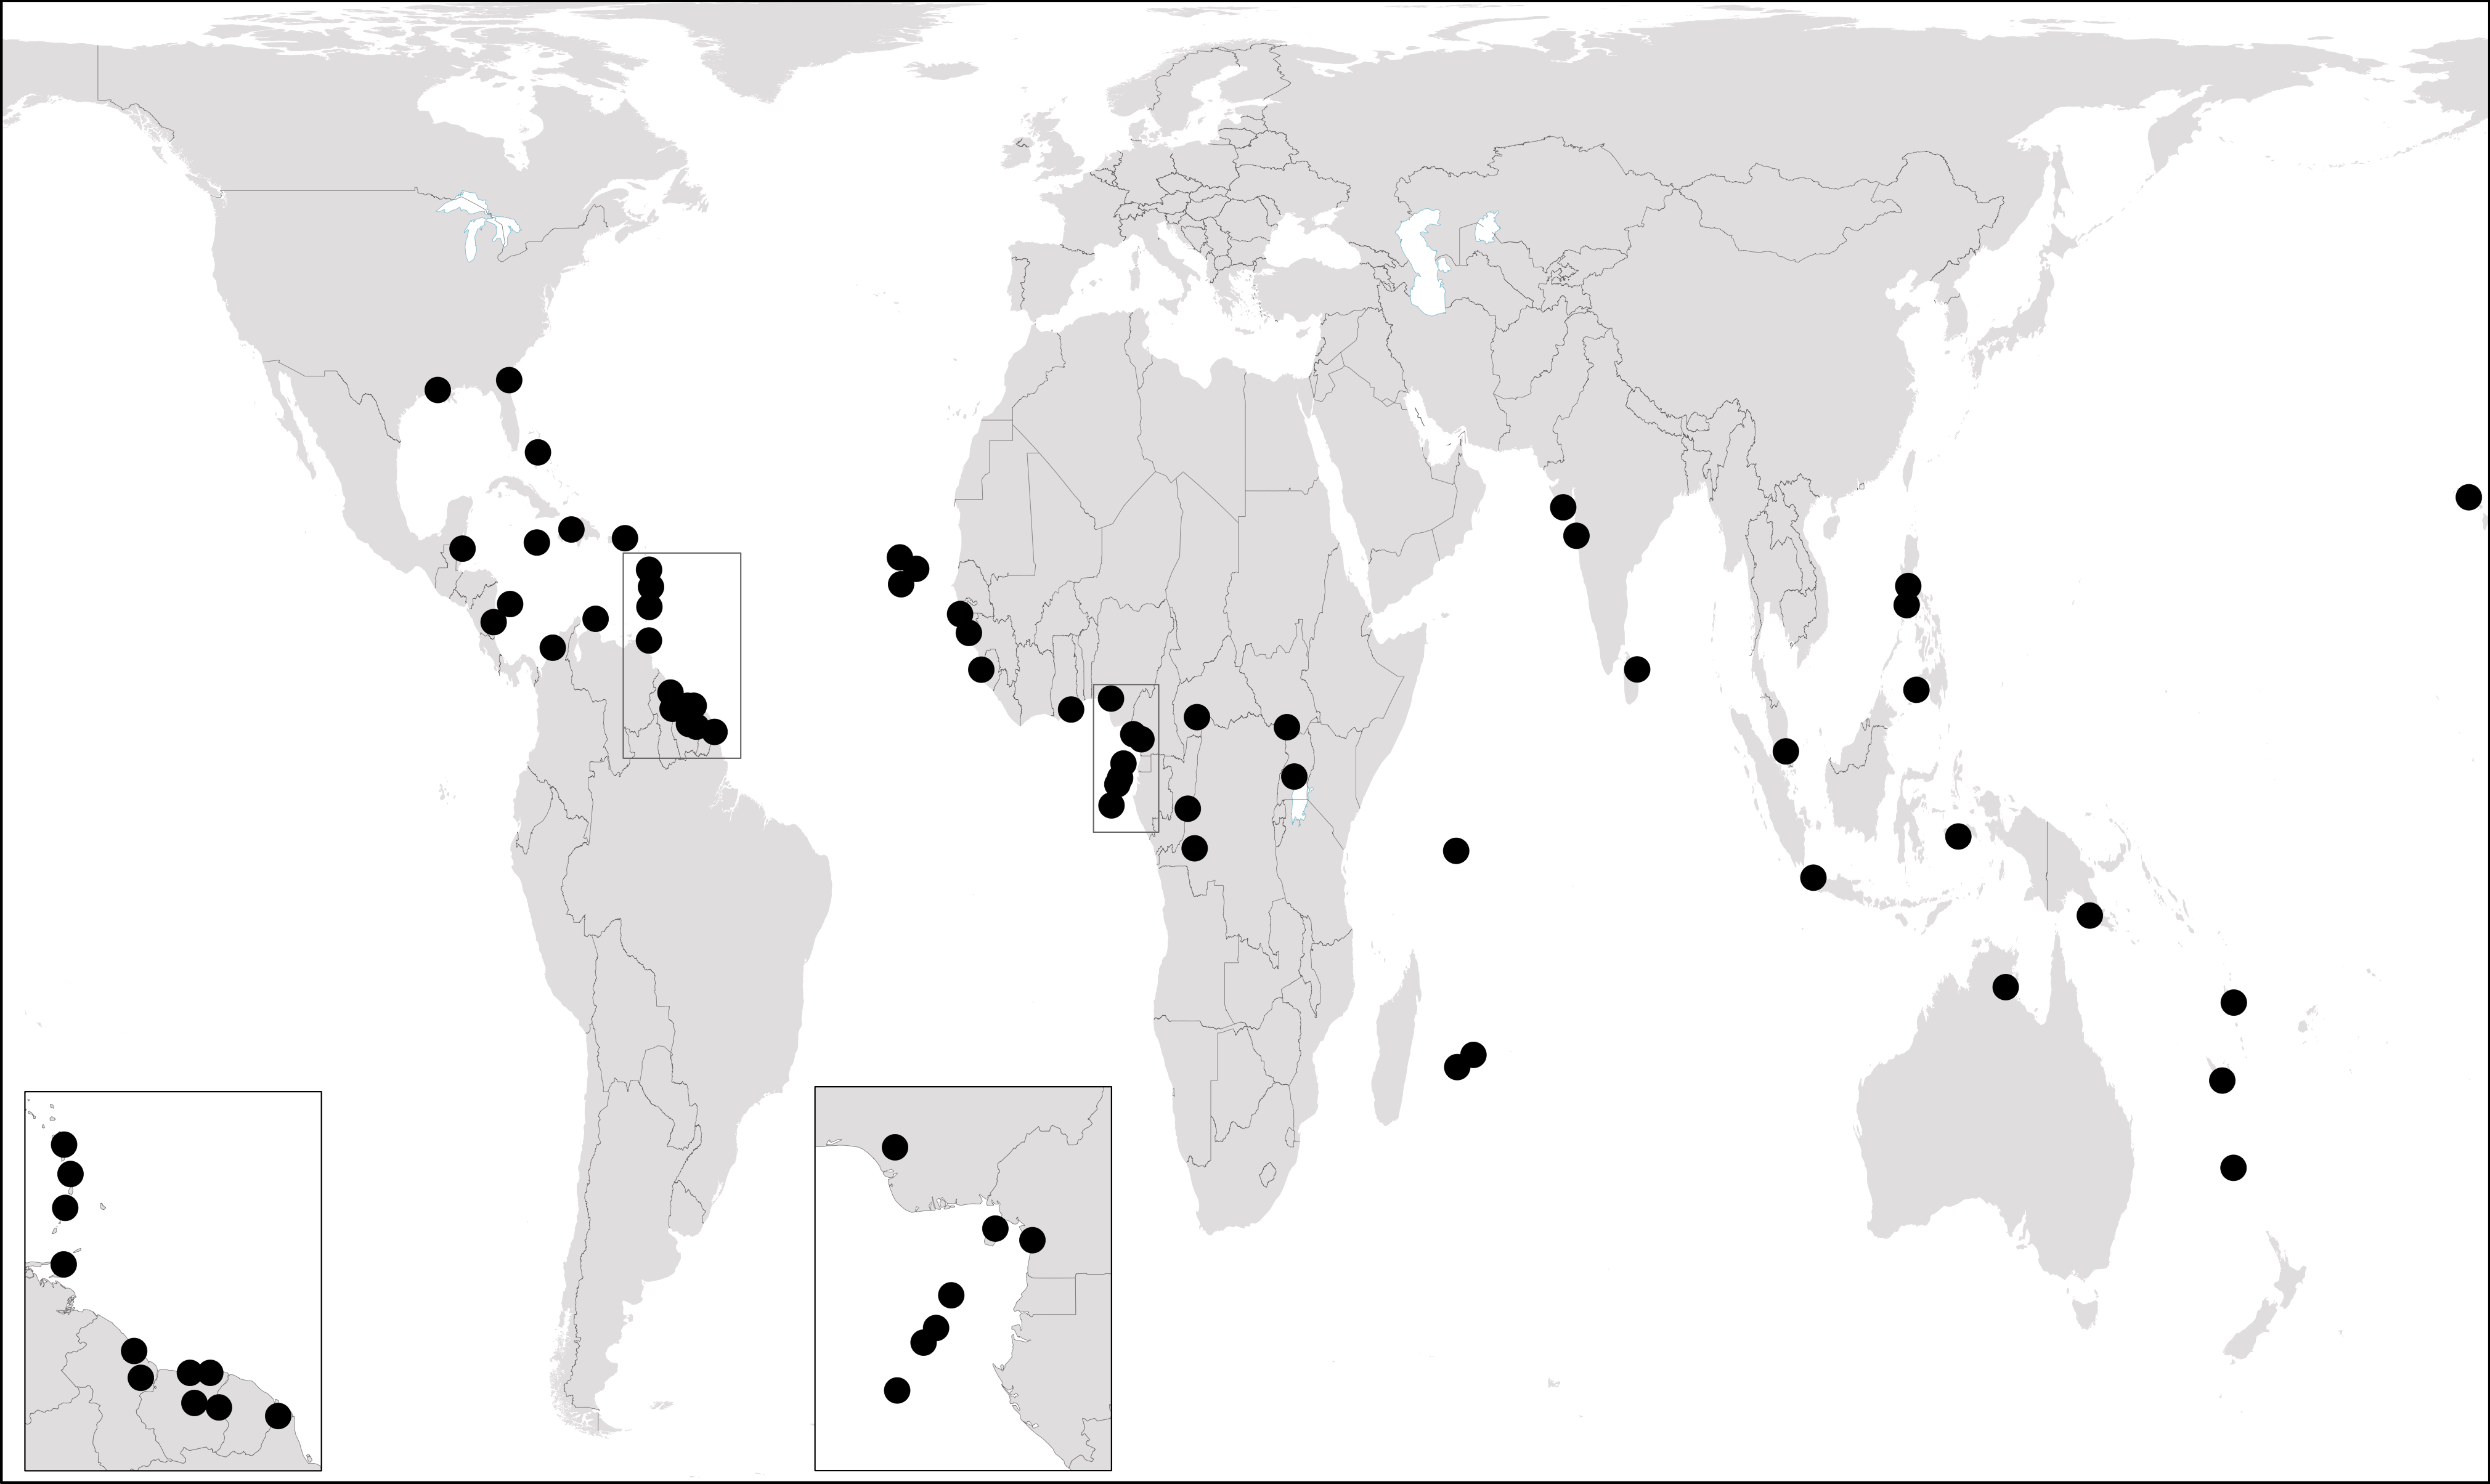
\includegraphics[width=\textwidth]{figures/Michaelis-Fig1.png}
\caption{Distribution of the 59 creole languages in APiCS (for more information see apics-online.info) (CC BY-SA 4.0, Hans-Jörg Bibiko, MPI-SHH/Jena)}
\label{fig:michaelis:1}
\end{figure}

% \begin{verbatim}%%move bib entries to  localbibliography.bib
% @article{Allen2002,
% 	author = {Allen, Cynthia L.},
% 	journal = {\textit{Language Sciences}},
% 	pages = {189–211},
% 	sortname = {Allen, Cynthia L.},
% 	title = {The development of `strengthened' possessive pronouns in {English}},
% 	volume = {24.},
% 	year = {2002}
% }
% 
% 
% @misc{Bentz2013,
% 	author = {Bentz, Christian  and  Bodo Winter},
% 	note = {Languages with more second language learners},
% 	year = {2013}
% }
% 
% 
% tend to lose nominal case. \textit{Language Dynamics and Change} 3. 1–27.
% 
% Bybee, Joan L. 2007. Introduction. In: Joan L. Bybee (ed.), \textit{Frequency of use and the organization of language}, 5–22. Oxford: Oxford University Press.
% 
% @incollection{Bybee2006,
% 	address = {Cambridge},
% 	author = {Bybee, Joan L.},
% 	booktitle = {\textit{Linguistic universals}},
% 	editor = {Ricardo Mairal and Juana Gil},
% 	pages = {179–194},
% 	publisher = {Cambridge University Press},
% 	sortname = {Bybee, Joan L.},
% 	title = {Language change and universals},
% 	year = {2006}
% }
% 
% 
% @incollection{Bybee1988,
% 	address = {Oxford},
% 	author = {Bybee, Joan L.},
% 	booktitle = {\textit{Explaining language universals}},
% 	editor = {John A. Hawkins},
% 	pages = {350–379},
% 	publisher = {Blackwell},
% 	sortname = {Bybee, Joan L.},
% 	title = {The diachronic dimension in explanation},
% 	year = {1988}
% }
% 
% 
% Colot, Serge \& Ludwig, Ralph. 2013. Martinican Creole structure dataset. In Susanne Maria Michaelis, Philippe Maurer, Martin Haspelmath \& Magnus Huber (eds.), \textit{Atlas of pidgin and creole language structures online.} Leipzig: Max Planck Institute for Evolutionary Anthropology. https://apics-online.info/contributions/36.
% 
% @incollection{Cristofaro2017,
% 	address = {Berlin},
% 	author = {Cristofaro, Sonia},
% 	booktitle = {\textit{Dependencies in language}},
% 	editor = {Nick J. Enfield},
% 	pages = {9–23},
% 	publisher = {Language Science Press},
% 	title = {Implicational universals and dependencies},
% 	year = {2017}
% }
% 
% 
% Cristofaro, Sonia. 2018 [this volume]. Taking diachronic evidence seriously: Result-oriented vs. source-oriented explanations of typological universals. In Karsten Schmidtke-Bode, Natalia Levshina, Susanne Maria Michaelis \& Ilja Seržant (eds.), \textit{Explanation in typology: Diachronic sources, functional motivations and the nature of the evidence}, . Berlin: Language Science Press.
% 
% @book{Croft1991,
% 	address = {Chicago},
% 	author = {Croft, William},
% 	publisher = {The University of Chicago Press},
% 	title = {\textit{Syntactic categories and grammatical relations: The cognitive organization of information}},
% 	year = {1991}
% }
% 
% 
% @book{Cyffer1998,
% 	address = {Cologne},
% 	author = {Cyffer, Norbert},
% 	publisher = {Köppe},
% 	title = {\textit{A sketch of {Kanuri}}},
% 	year = {1998}
% }
% 
% 
% Fattier, Dominique. 2013. Haitian structure data set. In Susanne Maria Michaelis, Philippe Maurer, Martin Haspelmath \& Magnus Huber (eds.), \textit{Atlas of pidgin and creole language structures online.} Leipzig: Max Planck Institute for Evolutionary Anthropology.
% 
% Finney, Malcolm Awadajin. 2013. Krio structure dataset. In Susanne Maria Michaelis, Philippe Maurer, Martin Haspelmath \& Magnus Huber (eds.), \textit{Atlas of pidgin and creole language structures online.} Leipzig: Max Planck Institute for Evolutionary Anthropology. https://apics-online.info/contributions/15
% 
% Hagemeijer, Tjerk. 2013. Santome structure dataset. In Susanne Maria Michaelis, Philippe Maurer, Martin Haspelmath \& Magnus Huber (eds.), \textit{Atlas of pidgin and creole language structures online}. Leipzig: Max Planck Institute for Evolutionary Anthropology. https://apics-online.info/contributions/35
% 
% @book{Haspelmath1993,
% 	address = {(Mouton Grammar Library 9). Berlin},
% 	author = {Haspelmath, Martin},
% 	publisher = {Mouton de Gruyter},
% 	title = {\textit{A grammar of {Lezgian}}},
% 	year = {1993}
% }
% 
% 
% @incollection{Haspelmath2008,
% 	address = {Oxford},
% 	author = {Haspelmath, Martin},
% 	booktitle = {\textit{Language universals and language change}},
% 	editor = {Jeff Good},
% 	pages = {185--214},
% 	publisher = {Oxford University Press},
% 	title = {Creating economical morphosyntactic patterns in language change},
% 	year = {2008}
% }
% 
% 
% @incollection{Haspelmath2015,
% 	address = {Berlin},
% 	author = {Haspelmath, Martin},
% 	booktitle = {\textit{{Egyptian}-Coptic linguistics in typological perspective}},
% 	editor = {Eitan Grossman, Martin Haspelmath and Tonio Sebastian Richter},
% 	pages = {103–143},
% 	publisher = {De Gruyter Mouton},
% 	title = {A grammatical overview of {Egyptian} and Coptic},
% 	year = {2015}
% }
%  
% 
% Haspelmath, Martin \& APiCS Consortium. 2013. Independent pronominal possessors. In Susanne Maria Michaelis, Philippe Maurer, Martin Haspelmath \& Magnus Huber (eds.), \textit{The atlas of pidgin and creole language structures}. Oxford: Oxford University Press, 150–3. http://apics-online.info/parameters/39.chapter.html.
% 
% @article{Haspelmath2014,
% 	author = {Haspelmath, Martin, Andreea Calude, Michael Spagnol, Heiko Narrog  and  Elif Bamyacı},
% 	journal = {\textit{Journal of Linguistics}},
% 	number = {3},
% 	pages = {587–625},
% 	sortname = {Haspelmath, Martin, Andreea Calude, Michael Spagnol, Heiko Narrog  and  Elif Bamyaci},
% 	title = {Coding causal-noncausal verb alternations: {{A}} form-frequency correspondence explanation},
% 	volume = {50},
% 	year = {2014}
% }
% 
% 
% @incollection{Haspelmath2017,
% 	address = {Amsterdam},
% 	author = {Haspelmath, Martin  and  Susanne Maria Michaelis},
% 	booktitle = {\textit{{{Europe}an} Perspectives {VI}: Selected Papers from the 8th International Conference on Language Variation in {Europe} ({ICL}a{VE} 8), \citealt{Leipzig2015}}},
% 	editor = {Isabelle Buchstaller and Beat Siebenhaar},
% 	pages = {3–22},
% 	publisher = {Benjamins},
% 	title = {Analytic and synthetic: {{T}}ypological change in varieties of {European} languages in Language Variation},
% 	year = {2017}
% }
% 
% 
% @misc{Jaeger2018,
% 	author = {Jaeger, T. Florian  and  Esteban Buz},
% 	note = {Signal reduction and linguistic encoding. \textit{Handbook of psycholinguistics.}},
% 	year = {2018}
% }
% 
% 
% @incollection{Koch2012,
% 	address = {Frankfurt/Main},
% 	author = {Koch, Peter  and  Wulf Oesterreicher},
% 	booktitle = {\textit{Communicative spaces}. \textit{Variation, contact, and change}. \textit{Papers in honour of {Ursula} Schaefer}},
% 	editor = {Claudia Lange, Beatrix Weber and Göran Wolf},
% 	pages = {441--473},
% 	publisher = {Lang},
% 	title = {Language of immediacy –~language of distance. {{O}}rality and Literacy from the perspective of language theory and linguistic history},
% 	year = {2012}
% }
% 
% 
% Kouwenberg, Silvia. 2013. Berbice Dutch. In Susanne Maria Michaelis, Philippe Maurer, Martin Haspelmath \& Magnus Huber (eds.), \textit{The survey of pidgin and creole languages}. \textit{Volume 1: English-based and Dutch-based languages}. Oxford: Oxford University Press.
% 
% @book{Kortmann2013,
% 	address = {\textit{The electronic world atlas of varieties of English.} Leipzig},
% 	editor = {Kortmann, Bernd \ and  Kerstin Lunkenheimer},
% 	note = {//ewave-atlas.org.},
% 	publisher = {Max Planck Institute for Evolutionary Anthropology. http:},
% 	sortname = {Kortmann, Bernd \ and  Kerstin Lunkenheimer},
% 	title = {\biberror{no title}},
% 	year = {2013}
% }
% 
% 
% @article{Lass1990,
% 	author = {Lass, Roger},
% 	journal = {\textit{Journal of Linguistics}},
% 	number = {1},
% 	pages = {79–102},
% 	title = {How to do things with junk: {{{E}}}xaptation in language evolution},
% 	volume = {26},
% 	year = {1990}
% }
% 
% 
% @article{Lass2017,
% 	author = {Lass, Roger},
% 	journal = {\textit{Exaptation and language change}. Amsterdam: John Benjamins, 2016. \textit{Diachronica} 34:},
% 	pages = {117–126},
% 	title = {Review of Muriel Norde \& Freek {Van} de Velde, eds},
% 	volume = {1.},
% 	year = {2017}
% }
% 
% 
% Luffin, Xavier. 2013. Kinubi structure dataset. In Susanne Maria Michaelis, Philippe Maurer, Martin Haspelmath \& Magnus Huber (eds.), \textit{Atlas of pidgin and creole language structures online}. Leipzig: Max Planck Institute for Evolutionary Anthropology. https://apics-online.info/contributions/63.
% 
% @misc{Lupyan2010,
% 	author = {Lupyan, Gary  and  Rick Dale},
% 	note = {Language structure is partly determined by social structure. \textit{PLoS ONE} 5. http://journals.plos.org/plosone/article?id=10.1371.},
% 	year = {2010}
% }
% 
% 
% Manfredi, Stefano \& Sara Petrollino. 2013. Juba Arabic structure dataset. In Susanne Maria Michaelis, Philippe Maurer, Martin Haspelmath \& Magnus Huber (eds.), \textit{Atlas of pidgin and creole language structures online}. Leipzig: Max Planck Institute for Evolutionary Anthropology. http://apics-online.info/contributions/64.
% 
% Maurer, Philippe. 2013. Angolar structure dataset. In Susanne Maria Michaelis, Philippe Maurer, Martin Haspelmath \& Magnus Huber (eds.), \textit{Atlas of pidgin and creole language structures online.} Leipzig: Max Planck Institute for Evolutionary Anthropology. https://apics-online.info/contributions/36.
% 
% @article{Meyer2008,
% 	author = {Meyer, Julien},
% 	journal = {\textit{Journal of the International Phonetic Association}},
% 	number = {1},
% 	pages = {69--94},
% 	title = {Typology and acoustic strategies of whistled languages: {{P}}honetic comparison and perceptual cues of whistled vowels},
% 	volume = {38},
% 	year = {2008}
% }
% 
% 
% @book{Meyer2005,
% 	address = {Lyon},
% 	author = {Meyer, Julien},
% 	publisher = {Université Lumière Lyon 2},
% 	title = {Description typologique et intelligibilité des langues sifflées, approche linguistique et bioacoustique, Doctoral Dissertation},
% 	year = {2005}
% }
% 
% 
% \begin{styleHTMLPreformatted}
% Meyerhoff, Miriam. 2013. Bislama structure dataset. In Susanne Maria Michaelis, Philippe Maurer, Martin Haspelmath \& Magnus Huber (eds.), \textit{Atlas of pidgin and creole language structures online.} Leipzig: Max Planck Institute for Evolutionary Anthropology. https://apics-online.info/contributions/23.
% \end{styleHTMLPreformatted}
% 
% \begin{styleHTMLPreformatted}
% @book{Michaelis2018,
% 	address = {In Andrej Malchukov \& Walter Bisang, \textit{Handbook of areal patterns of grammaticalization and cross-linguistic variation in grammaticalization scenarios}, Berlin},
% 	author = {Michaelis, Susanne Maria  and  Martin Haspelmath},
% 	publisher = {De Gruyter Mouton},
% 	title = {Grammaticalization in creole languages: {{A}}ccelerated functionalization and semantic imitation},
% 	year = {2018}
% }
% 
% \end{styleHTMLPreformatted}
% 
% @book{Michaelis2013,
% 	address = {Oxford},
% 	booktitle = {\textit{The atlas of pidgin and creole language structures}},
% 	editor = {Michaelis, Susanne Maria, Philippe Maurer, Martin Haspelmath \ and  Magnus Huber},
% 	publisher = {Oxford University Press},
% 	sortname = {Michaelis, Susanne Maria, Philippe Maurer, Martin Haspelmath \ and  Magnus Huber},
% 	title = {\textit{The atlas of pidgin and creole language structures}},
% 	year = {2013}
% }
% 
% 
% @article{Napoli2014,
% 	author = {Napoli, Donna Jo, Nathan Sanders  and  Rebecca Wright},
% 	journal = {\textit{Language}},
% 	number = {2},
% 	pages = {424–456},
% 	title = {On the linguistic effects of articulatory ease, with a focus on sign languages},
% 	volume = {90},
% 	year = {2014}
% }
% 
% 
% Neumann-Holzschuh, Ingrid  \& Thomas A. \citealt{Klingler2013}. Louisiana Creole structure dataset. In Susanne Maria Michaelis, Philippe Maurer, Martin Haspelmath \& Magnus Huber (eds.), \textit{Atlas of pidgin and creole language structures online}. Leipzig: Max Planck Institute for Evolutionary Anthropology. http://apics-online.info/contributions/53.
% 
% @article{Norcliffe2016,
% 	author = {Norcliffe, Elisabeth  and  T. Florian Jaeger},
% 	journal = {\textit{Language and Cognition}},
% 	number = {2},
% 	pages = {167–205},
% 	sortname = {Norcliffe, Elisabeth  and  T. Florian Jaeger},
% 	title = {Predicting head-marking variability in {Yucatec Maya} relative clause production},
% 	volume = {8},
% 	year = {2016}
% }
% 
% 
% @book{Norde2016,
% 	address = {Amsterdam},
% 	booktitle = {\textit{Exaptation and language change}},
% 	editor = {Norde, Muriel \ and  Freek Van de Felde},
% 	publisher = {Benjamins},
% 	sortname = {Norde, Muriel \ and  Freek Van de Felde},
% 	title = {\textit{Exaptation and language change}},
% 	year = {2016}
% }
% 
% 
% @book{Schwarze1988,
% 	address = {Tübingen},
% 	author = {Schwarze, Christoph},
% 	publisher = {Niemeyer},
% 	title = {\textit{{Grammatik} der italienischen {Sprache}}},
% 	year = {1988}
% }
% 
% 
% Schwegler, Armin. 2013. Palenquero structure dataset. In Susanne Maria Michaelis, Philippe Maurer, Martin Haspelmath \& Magnus Huber (eds.), \textit{Atlas of pidgin and creole language structures online.} Leipzig: Max Planck Institute for Evolutionary Anthropology. https://apics-online.info/contributions/48.
%  
% Steinkrüger, Patrick O. 2013. Zamboanga Chabacano. In Susanne Maria Michaelis, Philippe Maurer, Martin Haspelmath \& Magnus Huber (eds.), \textit{The survey of pidgin and creole languages}. \textit{Volume 2: Portuguese-based, Spanish-based, and French-based languages}. Oxford: Oxford University Press.
% 
% Yakpo, Kofi. 2013. Pichi structure dataset. In Susanne Maria Michaelis, Philippe Maurer, Martin Haspelmath \& Magnus Huber (eds.), \textit{Atlas of pidgin and creole language structures online.} Leipzig: Max Planck Institute for Evolutionary Anthropology. https://apics-online.info/contributions/19.
% 
% @book{Ye2017,
% 	address = {Independent and dependent possessive person forms},
% 	author = {Ye, Jingting},
% 	publisher = {\textstylegmail{A cross-linguistic study}. Talk at the Diversity linguistics seminar (21 \citealt{September2017}), Leipzig University},
% 	title = {\biberror{no title}},
% 	year = {2017}
% }
% 
% 
% \end{verbatim}
\end{document}